% Created 2018-11-26 月 22:17
% Intended LaTeX compiler: pdflatex
\documentclass[presentation,dvipdfmx,CJKbookmarks]{beamer}
\usepackage{CJKutf8}
\usepackage{atbegshi}
\AtBeginShipoutFirst{\special{pdf:tounicode UTF8-UTF16}} % for UTF-8
\usepackage[utf8]{inputenc}
\usepackage[T1]{fontenc}
\usepackage{graphicx}
\usepackage[export]{adjustbox}
\usepackage{lmodern}
\usepackage{grffile}
\usepackage{longtable}
\usepackage{wrapfig}
\usepackage{rotating}
\usepackage[normalem]{ulem}
\usepackage{amsmath}
\usepackage{textcomp}
\usepackage{amssymb}
\usepackage{capt-of}
\usepackage{hyperref}
 \usepackage{minted}
\usetheme{Boadilla}
\usecolortheme{crane}
\author{Bao Haojun}
\date{2015-11-20}
\title{Programming by Wishful Thinking}
\hypersetup{
 pdfauthor={Bao Haojun},
 pdftitle={Programming by Wishful Thinking},
 pdfkeywords={},
 pdfsubject={},
 pdfcreator={Emacs 26.1 (Org mode 9.1.9)}, 
 pdflang={English}}
\begin{document}
\begin{CJK*}{UTF8}{simsun}

\maketitle
\begin{frame}{Outline}
\tableofcontents
\end{frame}

\CJKtilde

\begin{enumerate}
\item Wishful Thinking
\label{sec:orgcdfff0a}

\begin{frame}[fragile,label={sec:orgf5d949d}]{SICP\thinspace 介绍(Structure and Interpretation of Computer Programs)}
 \begin{block}{怎么定义有理数及其各种运算?}
\end{block}
\begin{block}{很简单,假设我们有\thinspace 3\thinspace 个函数:\texttt{make-有理数},\texttt{取分母},\texttt{取分子}}
\end{block}
\begin{block}{举例:有理数乘法}
\begin{minted}[]{common-lisp}
(defun 有理数乘法 (有理数a 有理数b)
  (make-有理数
   (* (取分子 有理数a) (取分子 有理数b))
   (* (取分母 有理数a) (取分母 有理数b))))
\end{minted}
\end{block}
\end{frame}

\begin{frame}[label={sec:orgf156ef9}]{Get Things Done\thinspace 工作方法}
\begin{itemize}
\item Coders at Work\thinspace 中对\thinspace jwz\thinspace 的采访

“我就是列个单子,然后一项一项的划掉”

\begin{center}

\includegraphics[width=3cm]{./jwz.ps}
\end{center}

\item org-mode\thinspace 演示(agenda\thinspace 功能)

\begin{center}

\includegraphics[width=3cm]{./org-mode.ps}
\end{center}
\end{itemize}

\begin{block}{hello world}
\end{block}
\end{frame}
\begin{frame}[label={sec:org9d17340}]{Literate Programming}
\begin{itemize}
\item Knuth\thinspace 的工作方法

\begin{center}
\includegraphics[height=3cm]{./knuth.ps}
\end{center}

\item org-mode\thinspace 演示(knuth-mode)

\begin{center}

\includegraphics[width=3cm]{./org-mode.ps}
\end{center}
\end{itemize}
\end{frame}

\item Flow
\label{sec:orgdce52fd}
\end{enumerate}
\end{CJK*}
\end{document}
